\chapter{系统设计与架构}
跨界服务将跨越不同行业、组织、价值链等边界的服务进行深度融合和模式创新,为用户提供多维度、高质量、富价值的跨界服务,成为现代服务业发
展的重要创新途径。跨界服务平台是各类跨界服务集成的支撑系统,相比传统的服务集成,跨界服务融合需开展模式、生态、环境、质量、价值等多维深度融合。
为将提出的算法与应用相结合,本文依托于国家重点研发计划专项《现代服务业共性关键技术研发及应用示范》的子课题《跨界服务集成方法与支撑载体》,
在跨界服务平台设计并实现了服务智能调用引擎,本章主要对跨界服务平台和智能调用引擎进行介绍。

\section{跨界服务系统}
本文作者所在的课题组系统性地研究了跨界服务相关理论,并形成了跨界服务原型系统,
本节主要介绍系统整体架构以及跨界服务系统中两个核心模块服务交换机和服务路由器。

  跨界服务系统是针对跨界服务运行时呈现高维异构、复杂动态、开放分布的特点,解决跨界服务网络管理中高效接入、安
  全交换、智能路由等关键技术,形成的跨界服务集成工程化方法,研制软硬件结合的跨
  界服务集成及运行支撑载体,包括跨界服务集成设计软件套件、服务交换机与路由器硬
  件环境。

  海量跨界服务分布于服务网络中,不同服务之间相互操作,通过服务交换及路由技术,实现跨界服务的查找、调用
  及跨界服务间的交互,同时利用基于认证授权的开放服务安全交换技术,保证交换
  过程中的数据安全。服务交换机和服务路由器是支撑载体的关键,采用软硬结合
  的设计方案来实现,如图\ref{fig:system}所示,服务交换机实现跨界服务的高效接入、访问控制、消
  息映射、认证授权等功能,实现域内企业服务的安全可靠的开放,其架构包括设施层(机
  柜、电源、接口等)、设备层(计算服务器、存储服务器)、网络层(虚拟路由器、虚拟
  防火墙)、应用层(服务接入、访问控制、服务缓存等)。服务路由器提供服务聚合、
  服务查找、服务路由等能力,把异构服务联成网络,是跨界服务互联的基础设施,其架
  构包括设施层(机柜、电源、接口等)、设备层(计算服务器、存储服务器)、网络层(状
  态感知、消息路由等功能)、应用层(服务索引、服务查找、服务路由等)。

  \begin{figure}[htbp]
    \centering
    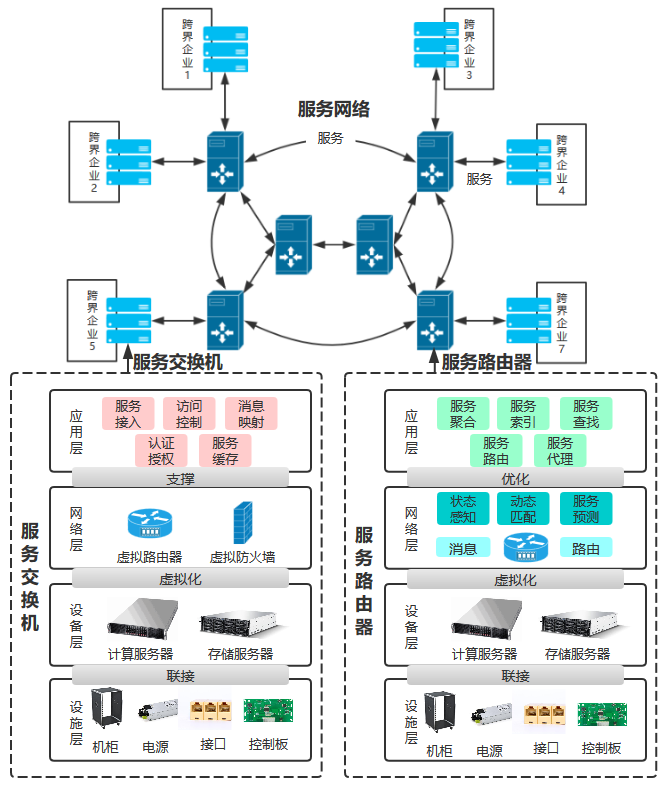
\includegraphics[width=10cm]{./images/system.png}
    \caption{JTangYdrail系统架构}
    \label{fig:system}
  \end{figure}

  服务交换机是跨界服务网络上最下层节点,
  使用服务地址在交换层接收并转发服务相关的数据,与实际服务直接相关,
  是服务的拥有者以及一次服务远程调用的发起者,
如图\ref{fig:switchboard}所示,主要包含以下几个模块:

1)The registry module :维护企业的服务信息和业务数据,
服务成功注册后,服务信息将存储在本地,并且其元数据将通过泛洪或其他方式广播到整个网络。
此后不久,其他服务交换机即可搜索和使用该服务交换机上服务。

2)The adapter module :旨在支持环境异构,AdM提供了各种适配器,可以通过不同的语言实现这些适配器,以实现与异构服务的通信。
在语义上兼容前提下,尽管硬件和软件平台,语言和API不同,但连接到不同适配器的各种服务在跨界服务系统仍将被连接和集成。

3)The policy module:使用多种策略来提高性能,代理策略使用户可以通过代理调用服务,服务交换机的负载平衡策略通过增加进程数来实现可伸缩性和负载平衡,
服务缓存策略使某些节点可以缓存服务调用的结果,从而可以充分利用网络中边缘节点的资源。 

4)The mapping module:旨在为用户带来便利,以特定格式调用服务或接收结果。
 提供了直观的图形界面,供用户生成规则文件。 
 
5)The authentication module:是基于密钥加密技术设计的,并使用基于角色的访问控制策略来保护数据的安全性。

  \begin{figure}[htbp]
    \subfloat[JTangYdrail 服务交换机软件架构]{
      \centering
      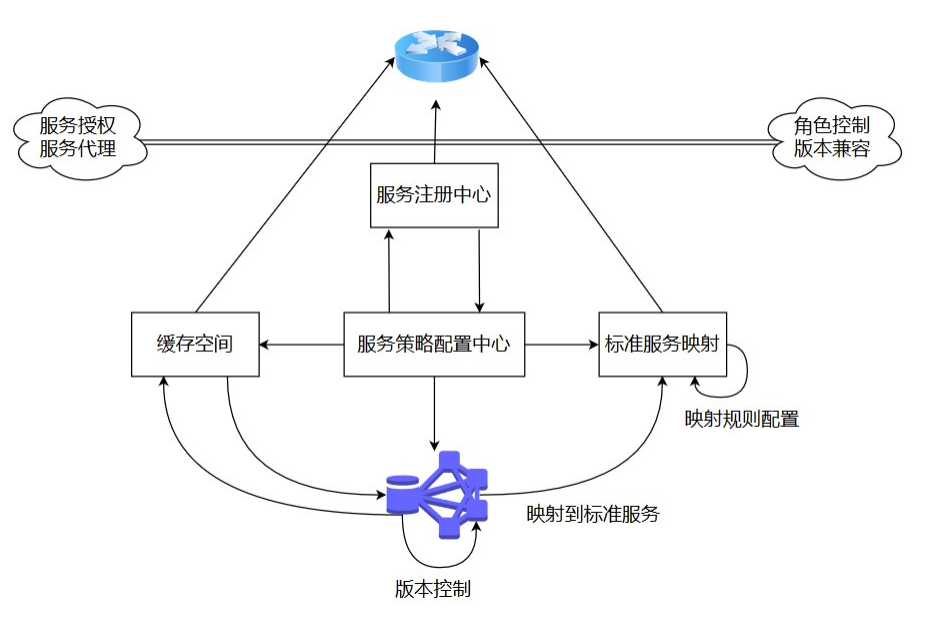
\includegraphics[width=8cm]{./images/switchboard.png}
      \label{fig:switchboard}
    }
    \subfloat[JTangYdrail 服务路由器软件架构]{
      \centering
      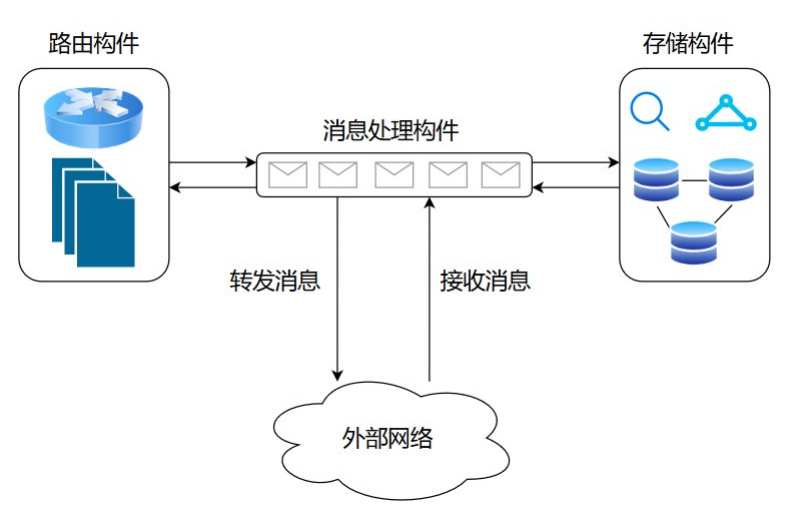
\includegraphics[width=8cm]{./images/router.png}
      \label{fig:router}
    }
    \caption{服务交换机和服务路由器架构}
    \label{fig:loss}
    \end{figure}


    服务路由器是在服务网络中转发服务元信息的网络设备,一方面,服务路由器从服务交换机收集服务信息,并在整个网络中广播数据。 
    另一方面,如果用户调用服务,则服务路由器会将请求转发到相应的服务节点。 
    服务路由器的结构如图\ref{fig:router}所示,其中包含路由组件,存储组件,处理器组件等:

    1)The storage component:由三部分组成:服务缓存,包括一些服务元数据和一些查询结果;
    路由信息,这是整个网络的基础,以及服务网络的结构信息。
    
    2)The routing component:功能是根据服务ID转发服务请求,该服务ID与传统网络中的IP地址完全不同。
    
    3)The processor component:提供内部和外部资源之间的通信机制。消息有两种类型:服务消息和路由消息。
    一旦收到消息,它将由PrC进行预处理,然后传输到路由组件或存储组件。
    
    4)The standardized service component:标准化服务组件设计用于服务网络中功能相似的同类服务,
    当发现Web服务的任何故障时,它可以通过使用标准化服务动态地将服务替换为合适的服务,从而大大提高了服务的可用性和可靠性。


  
  
  
\section{服务智能调用引擎}
上一节介绍了跨界服务系统,是本文主要依托的平台,本节在系统中提出了以语义理解模块为核心的服务智能调用引擎,基于此实现本文算法与应用的结合。
在跨界服务网络中,所有的服务都部署在服务交换机上,因此服务智能调用引擎也运行在服务交换机系统内。
服务智能调用引擎集成在服务交换机系统内运行在跨界服务网络中,因此智能调用的能力是在后端的,与用户使用的终端系统解耦,最终在服务端暴露智能调用的接口供
跨界服务网络的使用者选择。

\begin{figure}[htbp]
  \centering
  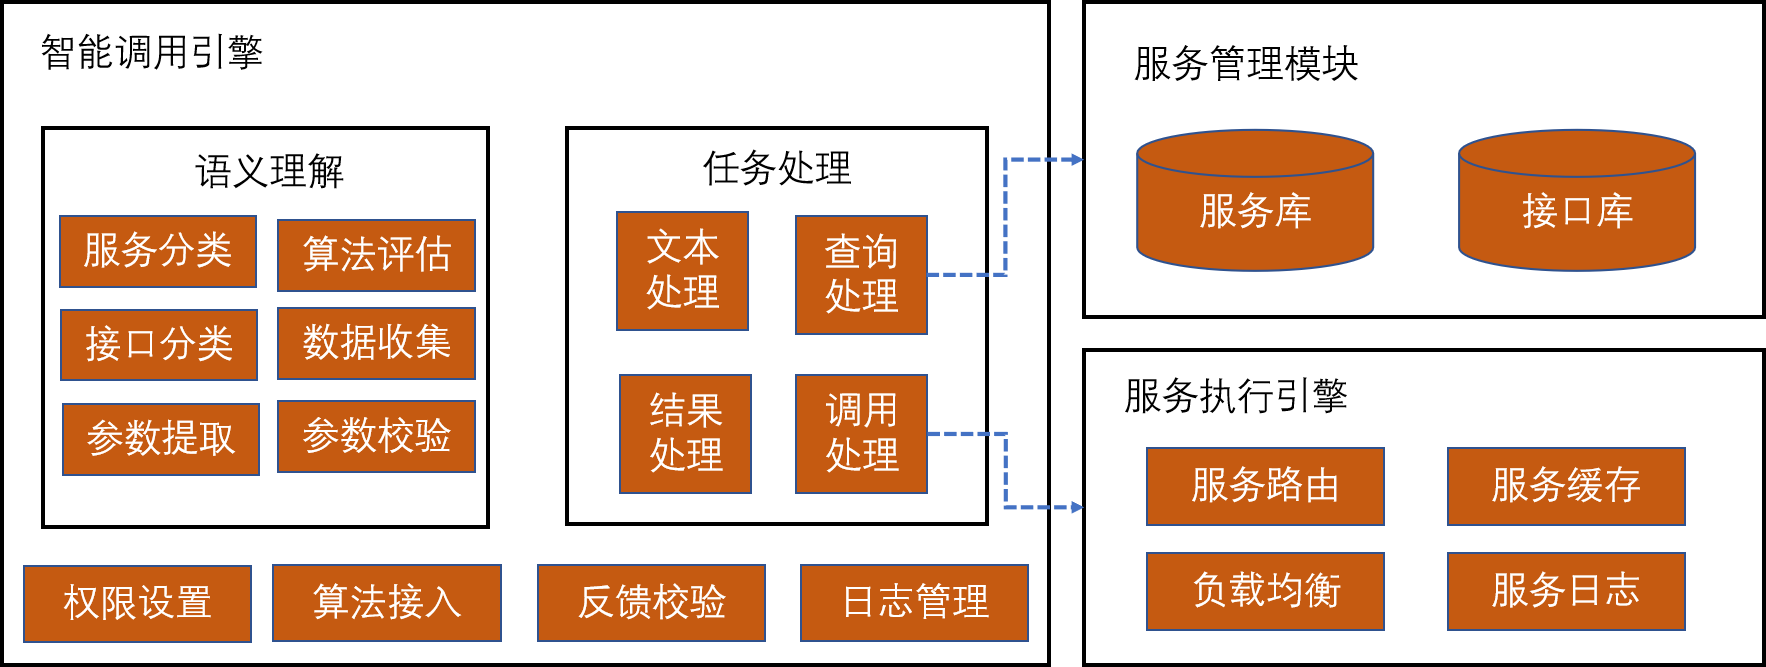
\includegraphics[width=15cm]{./images/yinqing.png}
  \caption{服务智能调用引擎架构}
  \label{fig:yinqing}
\end{figure}

如图\ref{fig:yinqing}所示,服务智能调用引擎主要包含语义理解和任务调度两个模块:

(1)语义理解:核心任务是本文一致在讨论的三项任务服务分类、接口分类和参数填充,接收的是用户输入的一句有目的性的话,识别用户的意图,根据
用户意图匹配相应的服务以及匹配该服务要执行的操作,找到匹配的服务以后,从用户输入的语句中提取在服务执行前需要
的执行参数,该模块算法采用的是实验性能最优的BERT-co-interactive模型。此外我们增加了数据收集模块,在每次调用之后,引擎会自动收集本次输入的语句作为数据保存,
以此来丰富平台的数据集,同时我们计划定期人工评估算法准确率进而优化模型。

(2)任务调度:该模块主要智能调用需要解决的工程问题,使引擎能与跨界服务平台结合。文本处理器主要做了边界字符和停用词过滤处理,处理好的语句传入模型输入层,模型识别
出本次服务调用需要的服务、接口和参数信息后,会首先通过查询处理器向系统中服务管理模块按关键字查询得到被调用服务在系统中的执行逻辑,这里会有一个校验逻辑,校验
内容包括调用者的权限合法性以及参数信息是否有误等,校验通过以后,调用处理器会带着必要的各项参数向服务执行引擎发送引擎,在跨界服务网络中找到服务源完成本次
服务的调用并返回结果到结果处理器,经结果处理器封装的最终结果会返回给用户。

\section{系统原型展示}
在跨界服务理论基础上,实现了跨界服务网络平台的原型系统,系统被命名为JTangYdrail(图\ref{fig:logo})。
跨界服务网络与支撑载体系统依托于课题《跨界服务集成方法与支撑载体》,包含跨界服务交换机子系统、跨界服务路由器子系统和
跨界服务网络子系统。通过跨界服务交换机子系统,可以实现企业服务的包装、开放、部署和管理,并提供相关原生工具;通过跨界服务路由器
子系统,可以实现服务路由器的管理与可视化监控,实时掌握当前路由器的运行情况;通过跨界网络子系统,可以实现对全局
所有自网络及其关联的服务交换机和服务路由器的动态监控,并可对子网络进行管理。

\begin{figure}[htbp]
  \subfloat[JTangYdrail 首页]{
    \centering
    
\includegraphics[width=8cm]{./images/ketisan.png}
    \label{fig:ketisan}
  }
  \subfloat[JTangYdrail logo]{
    \centering
  
\includegraphics[width=8cm]{./images/jianmu.jpg}
  \label{fig:logo}
  }
  \caption{JTangYdrail总览}
  \end{figure}
  如图所示,JTangYdrail系统主要包含服务交换机管理、服务交换机工具和服务智能调用三个模块\ref{fig:sangemokuai}。
  服务交换机管理模块是系统的核心部分,主要包括服务管理,流程管理,申请管理和用户管理等功能,管理跨界服务网络中与服务相关
  的所有信息;服务交换机工具工具模块包括标注服务映射,物联网服务,服务包装等功能,这些功能均以工具形式嵌入JTangYdrail系统,
  是系统的附加能力;服务智能调用是与本文相关的模块,在跨界服务网络中暴露智能调用的能力,对用户输入的语句识别后智能执行相应的服务。

  \begin{figure}[htbp]
    \centering
    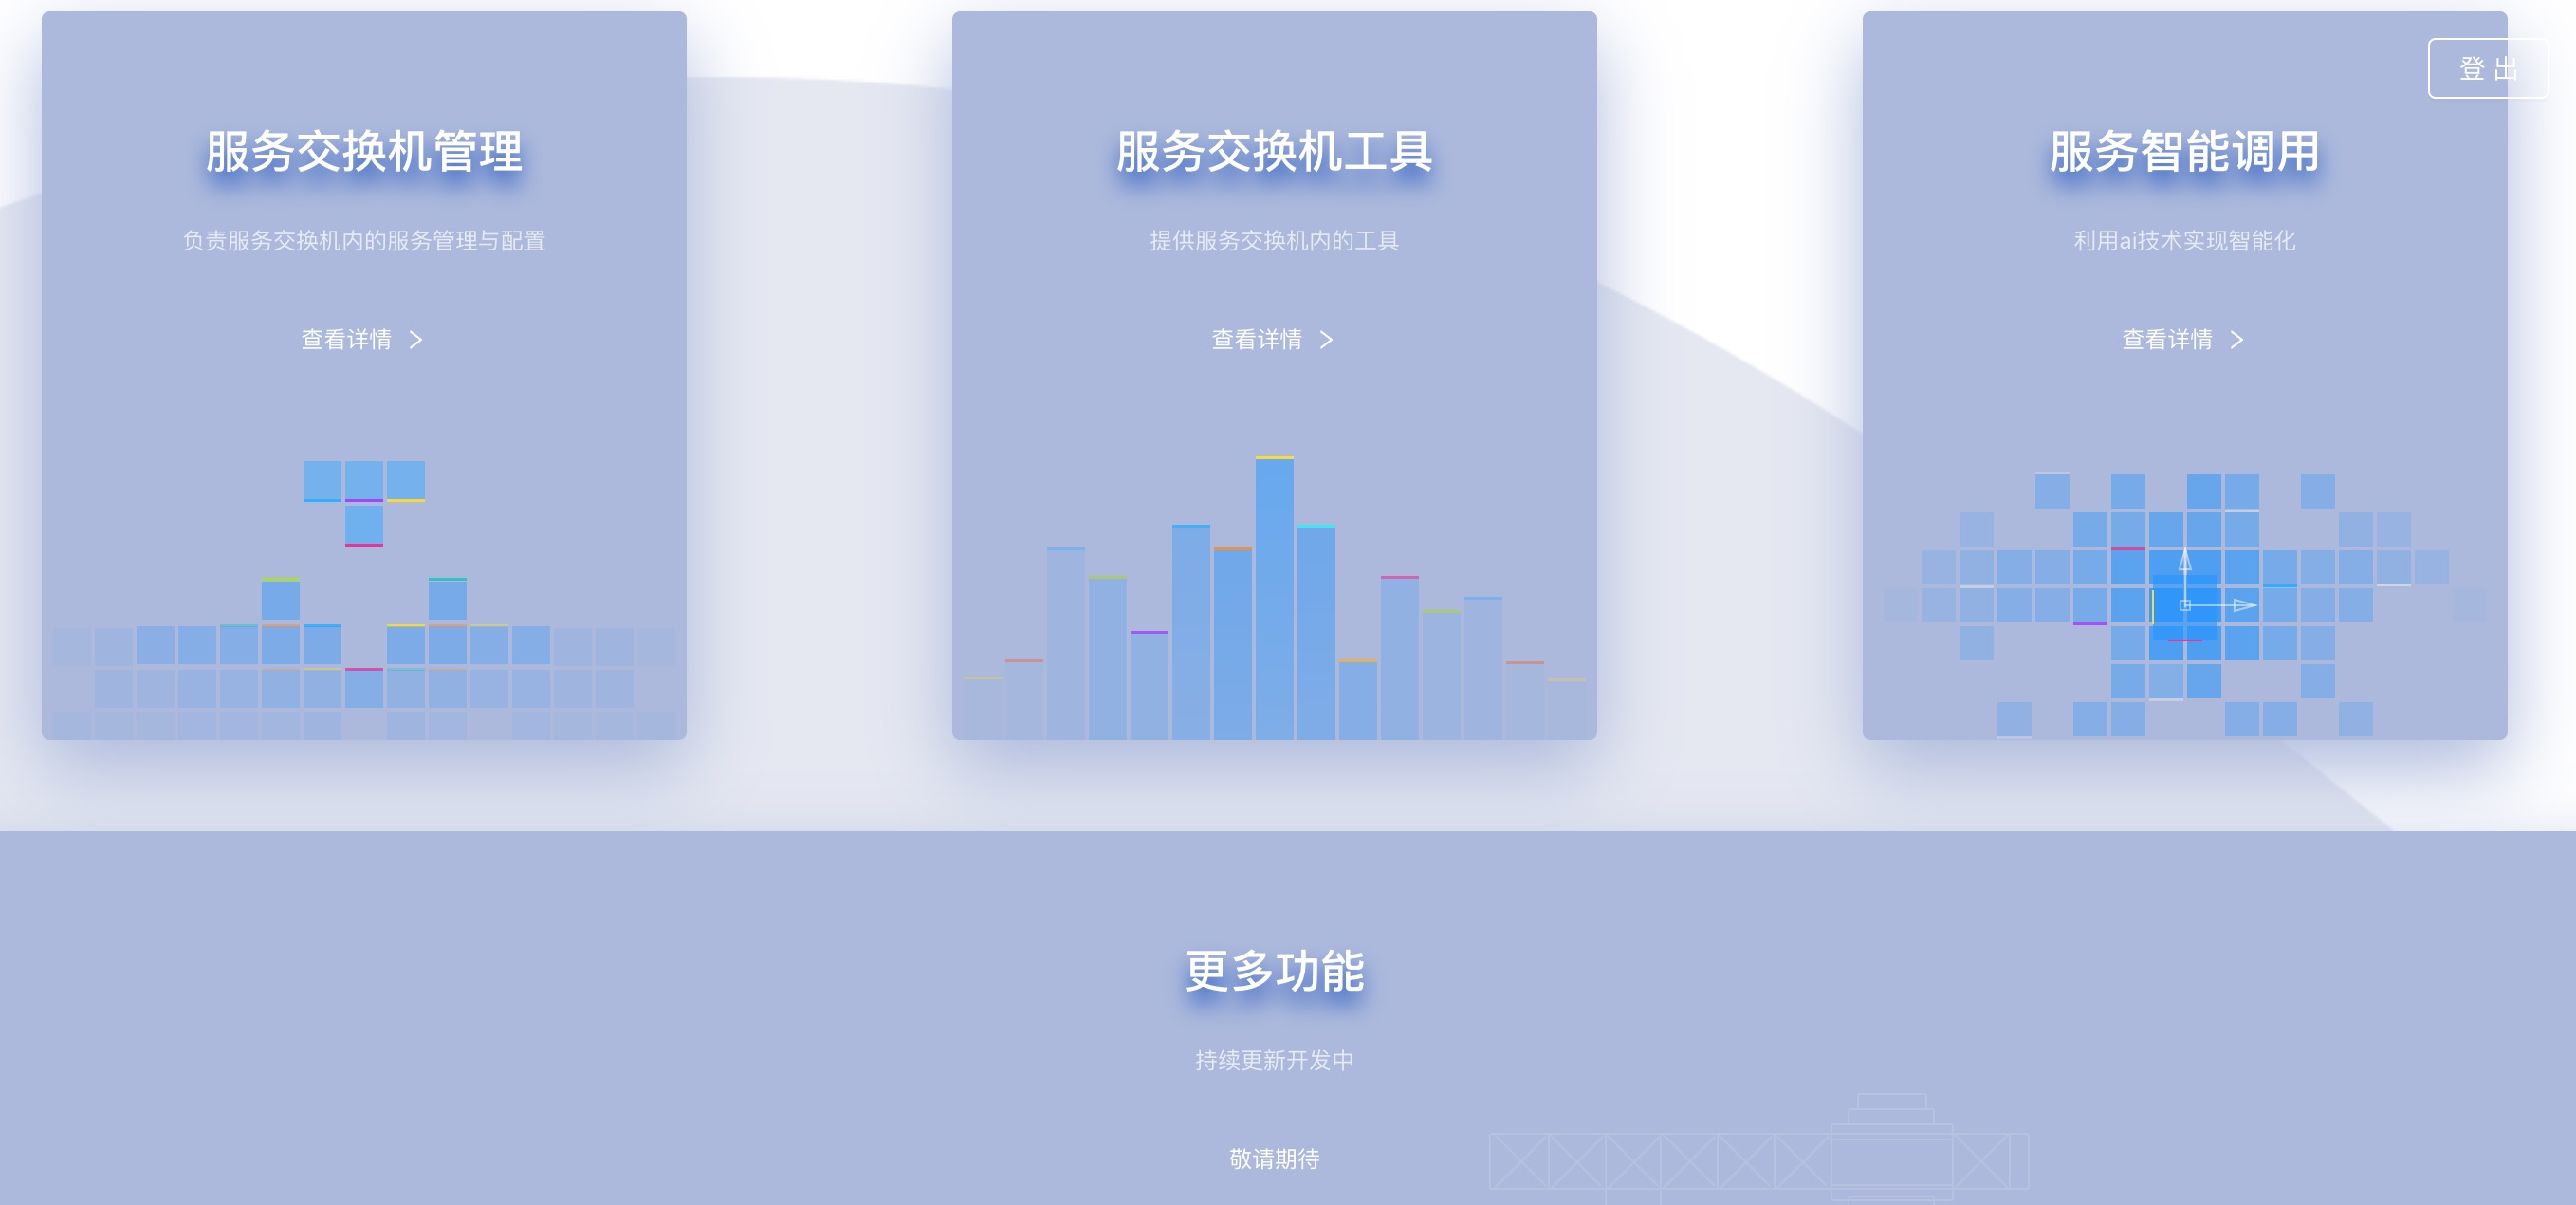
\includegraphics[width=17cm]{./images/sangemokuai.png}
    \caption{JTangYdrail 主要模块}
    \label{fig:sangemokuai}
  \end{figure}

\subsection{服务交换机管理模块}
本模块是系统的核心部分,进入系统后,点击服务详情页面对服务做CRUD,mapping,api management,test等一系列相关管理操作,
以及查看服务API的interface信息,parameter信息和SDK信息等。

如图\ref{fig:fuwuguanli}为服务管理模块的展示,服务管理的主要功能为: 
总览当前交换机内部所有服务的信息和实现对服务的增删改以及设置服务启用状态,
流程管理的主要功能为总览当前交换机内部所有流程的信息和实现对流程的增删改以及设置流程状态,
服务申请管理主要包含
企业对外进行服务申请需要的界面,可以申请其他服务交换机上的服务并实时反馈对方的审核信息,
部门管理的主要功能为
管理服务交换机中的各个部门,包括对部门信息的增删改查以及查看挂载在部门下的服务,
外部服务审批管理的主要功能为审核外部服务申请。
\begin{figure}[htbp]
  \subfloat[服务管理]{
    \centering
    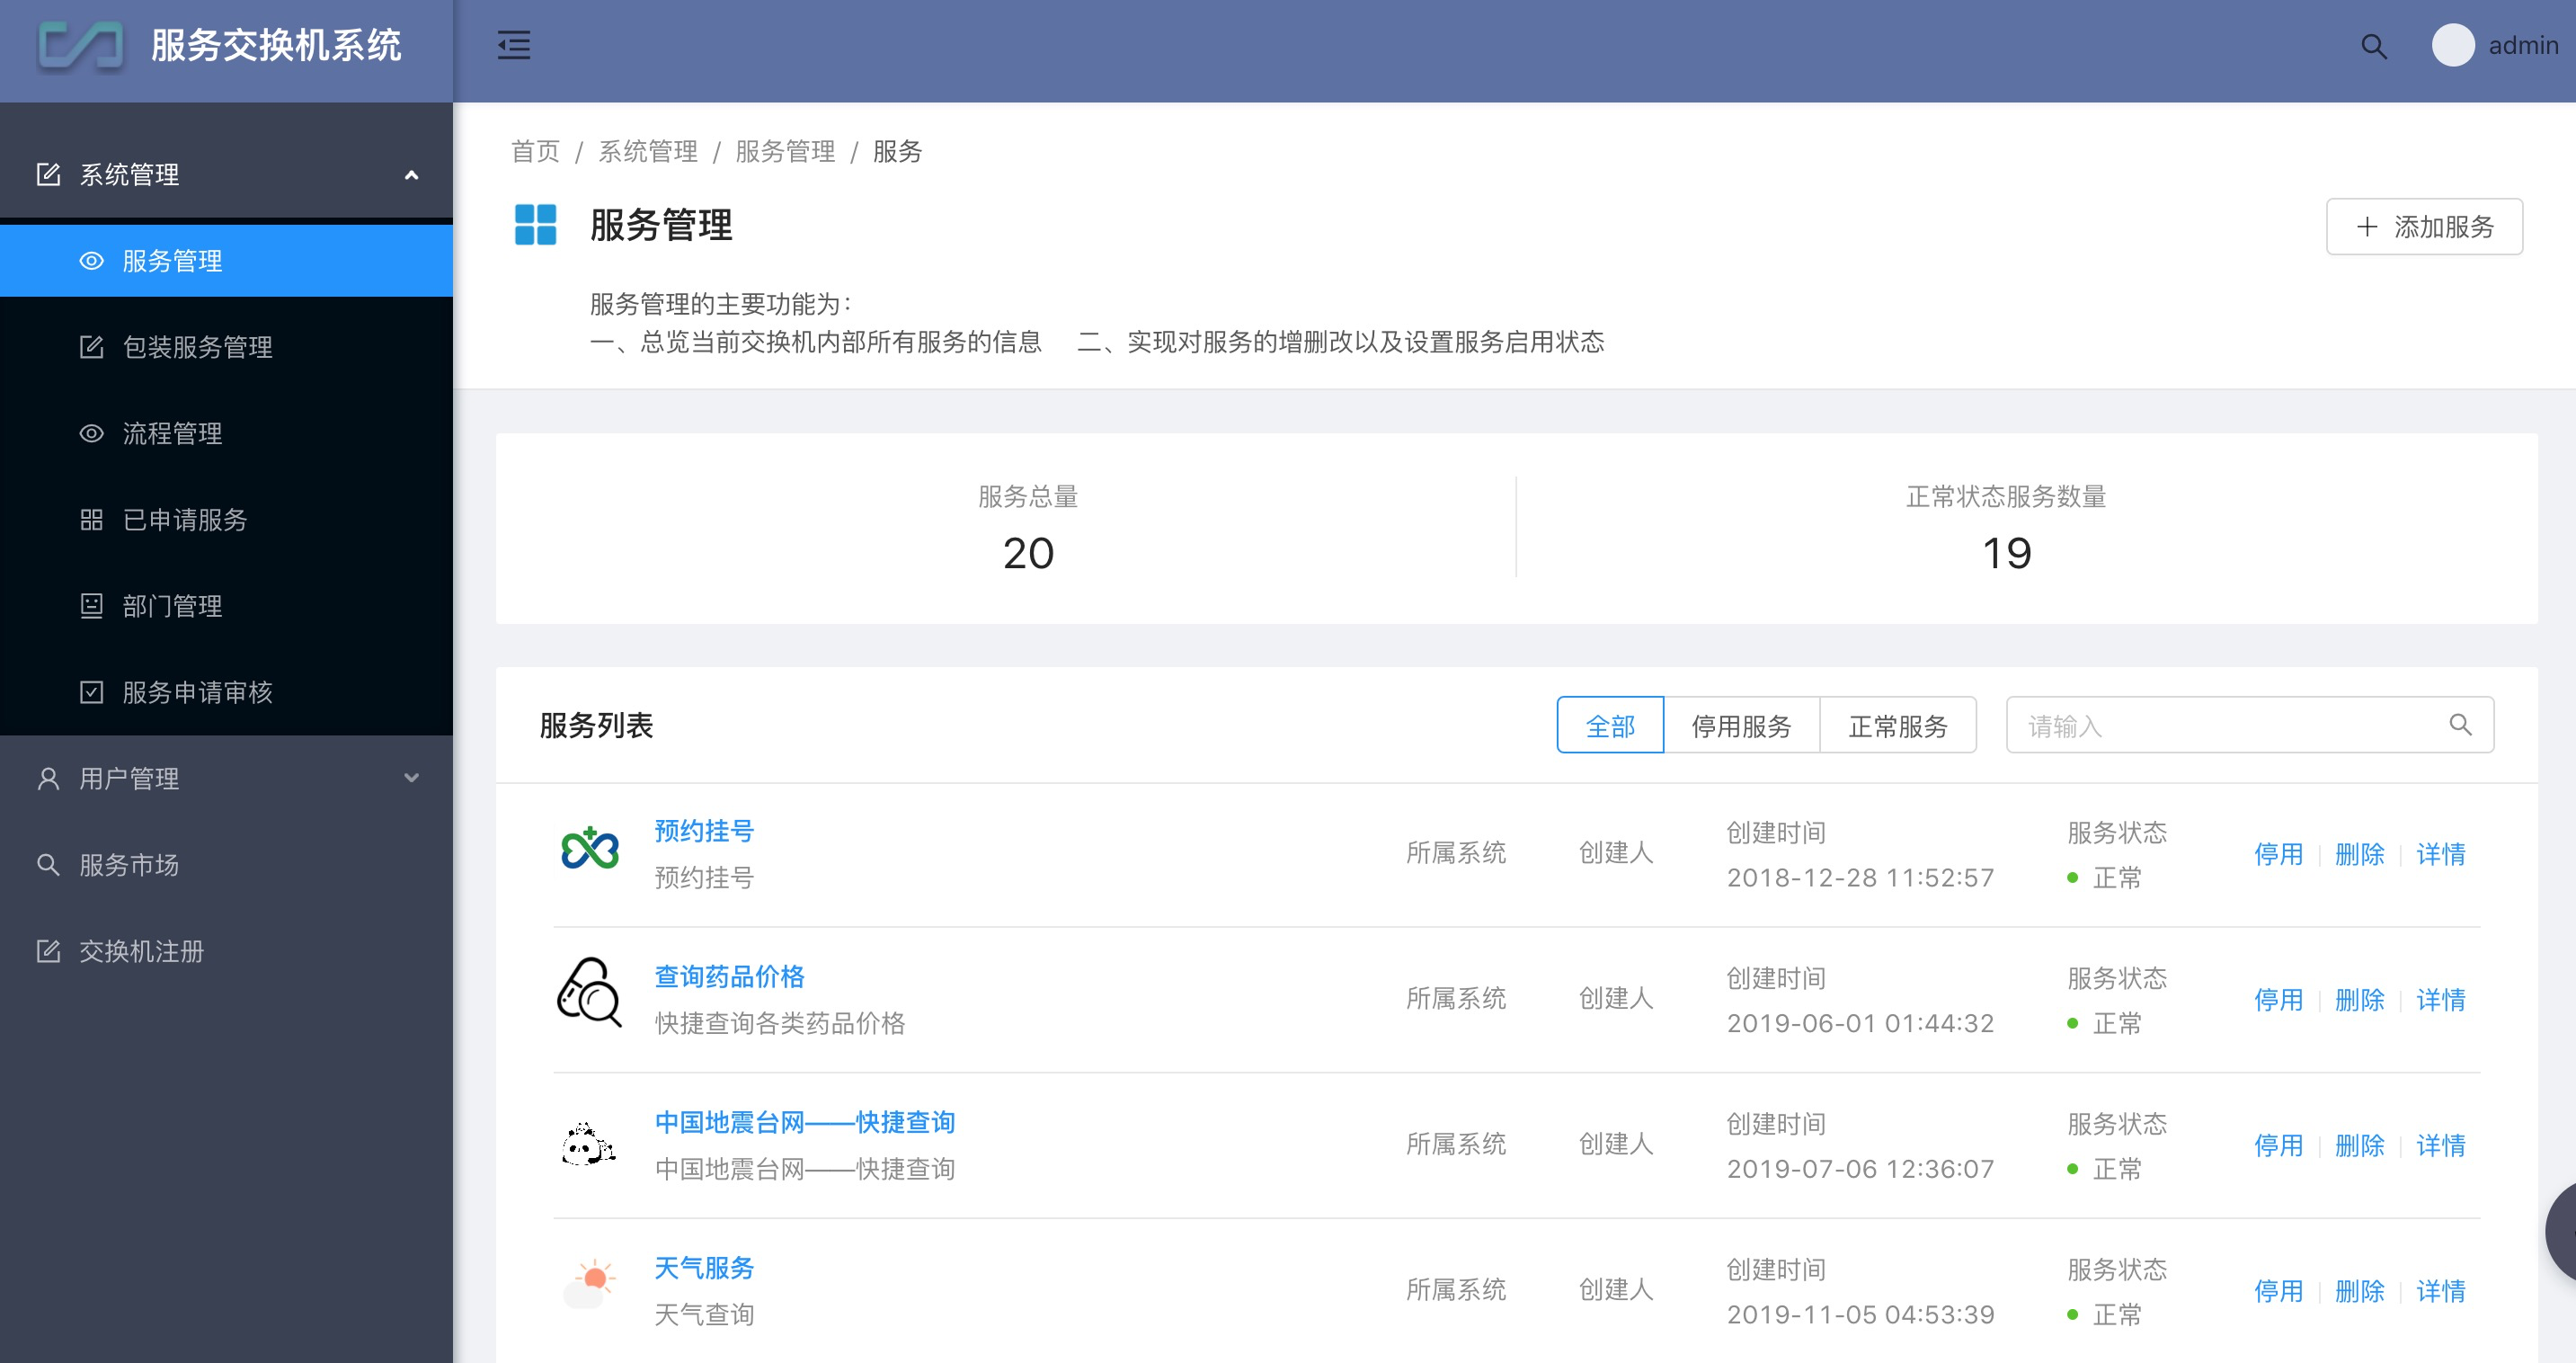
\includegraphics[width=8.3cm]{./images/fuwuguanli1.png}
    \label{fig:fuwuguanli1}
  }
  \subfloat[服务详情]{
    \centering
  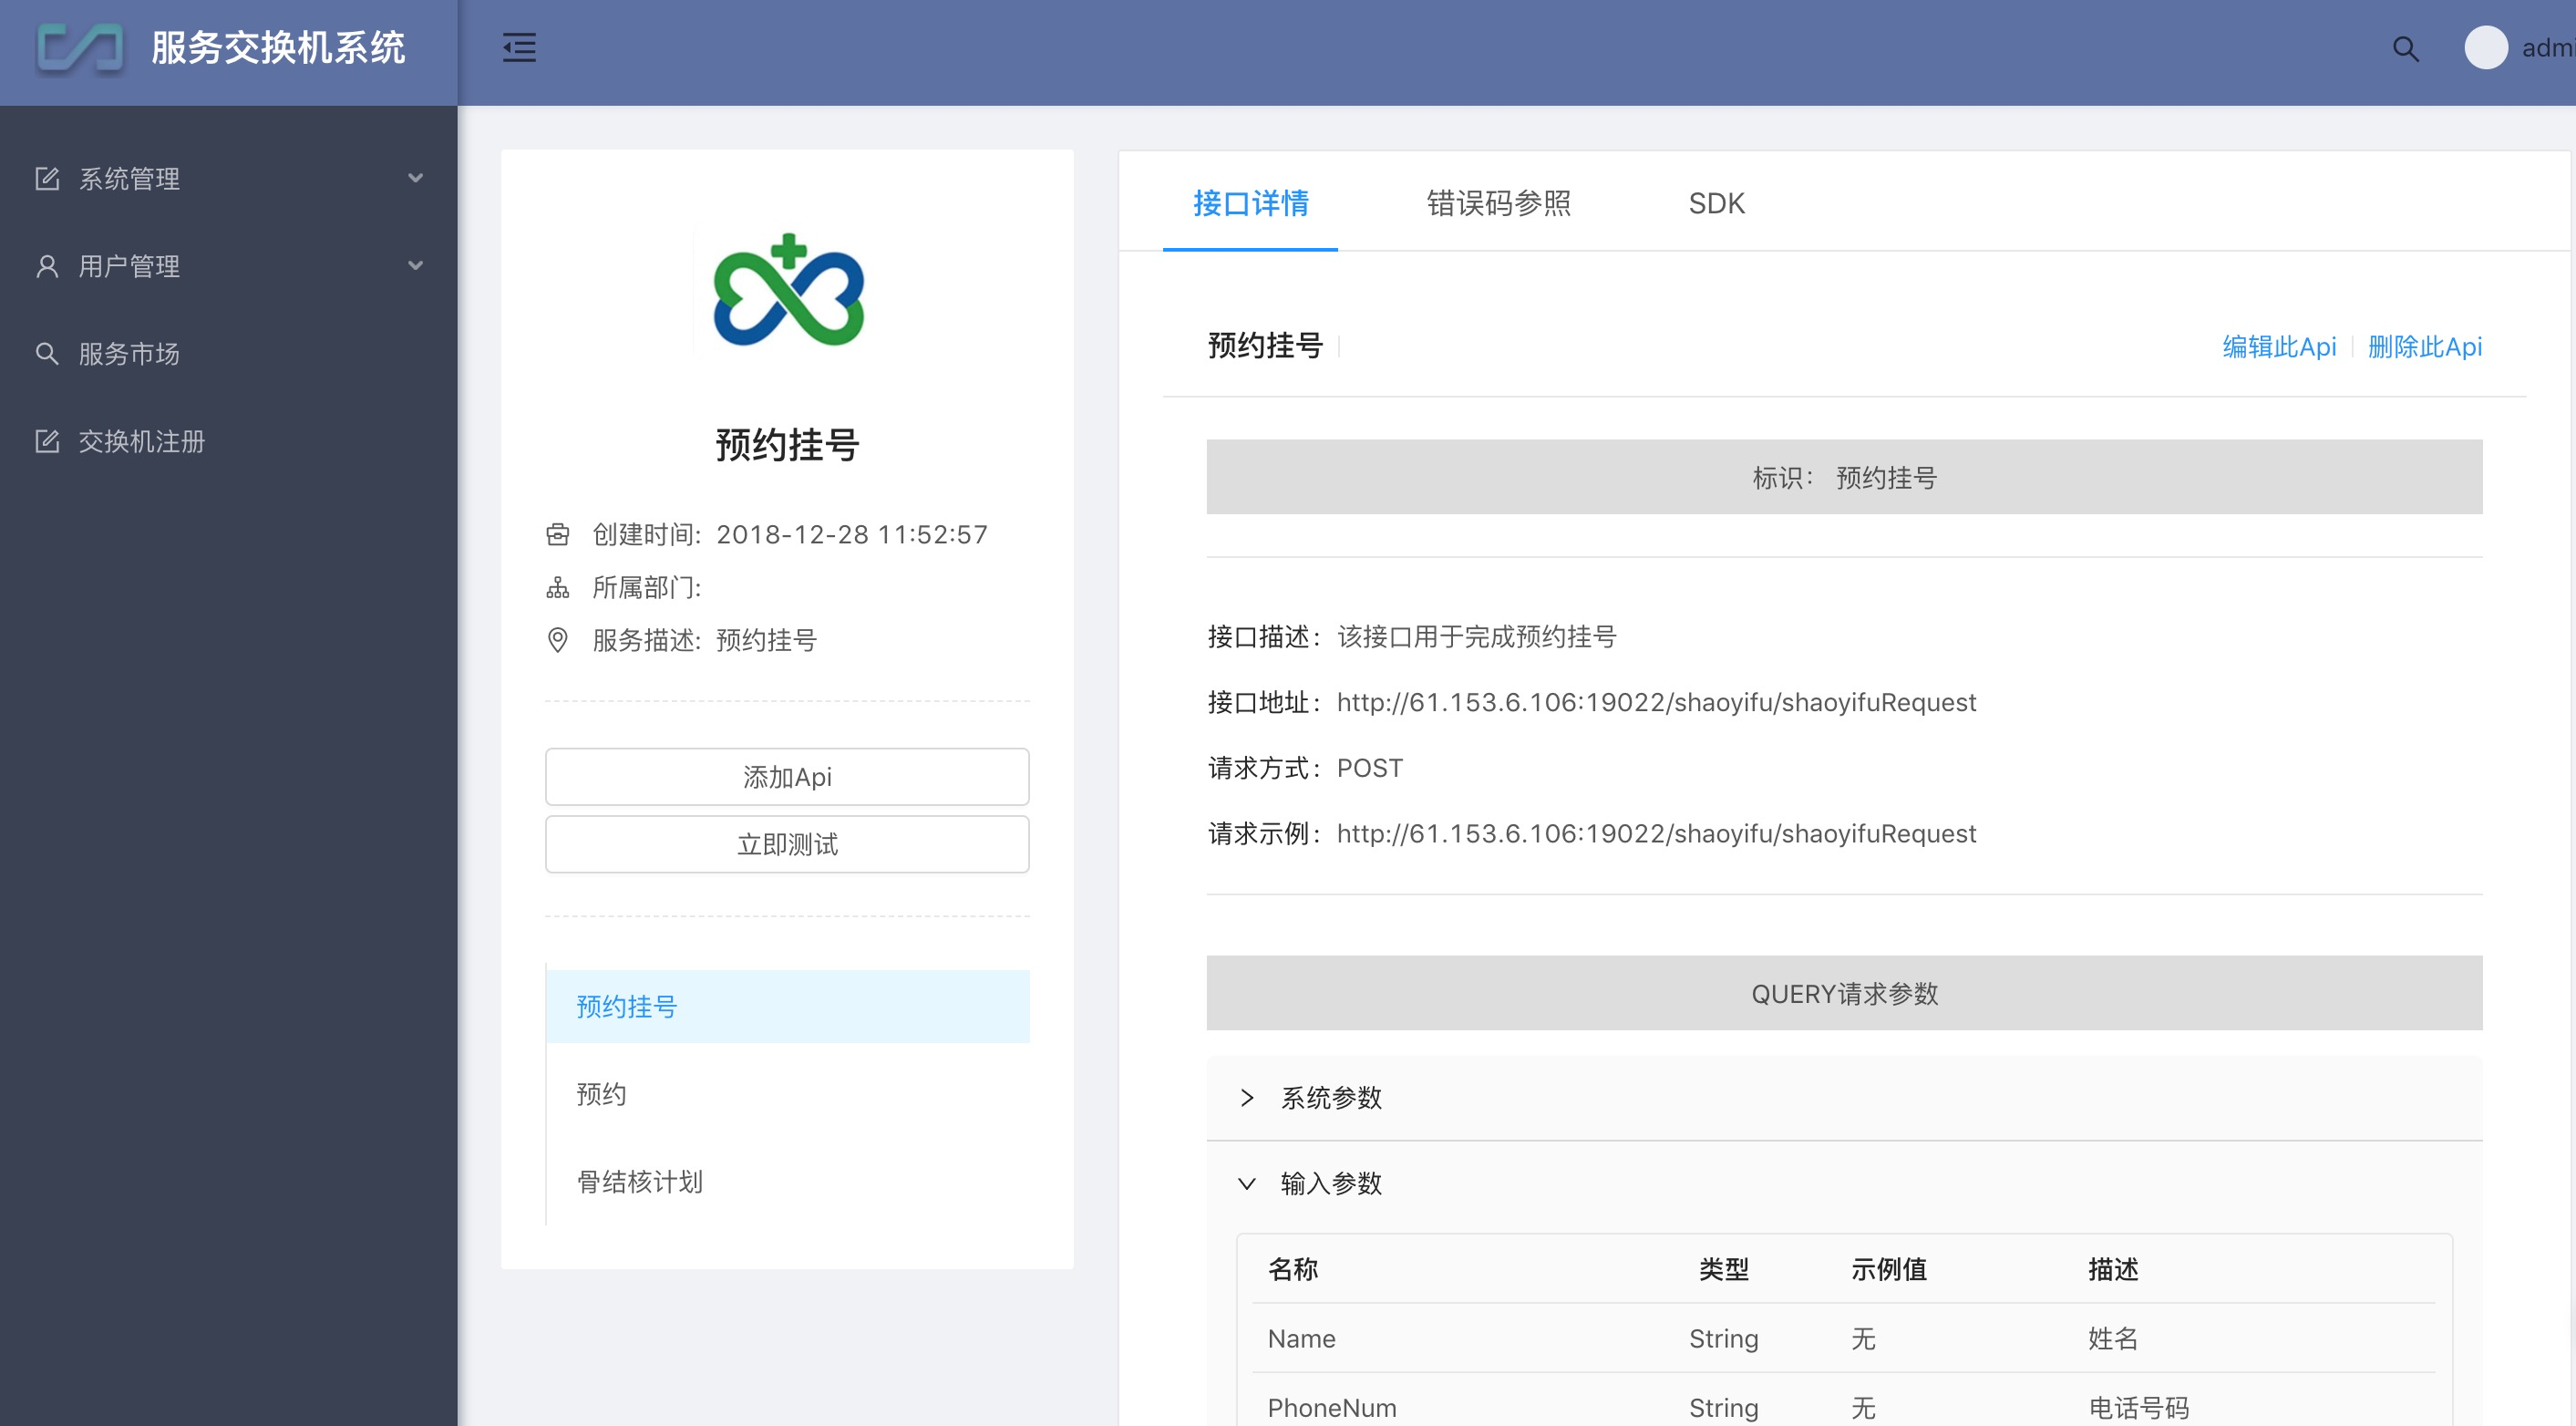
\includegraphics[width=8cm]{./images/fuwuguanli2.png}
  \label{fig:fuwuguanli2}
  }
  \caption{服务交换机管理模块}
  \label{fig:fuwuguanli}
  \end{figure}

  \subsection{服务交换机工具模块}
  本模块包括标准服务映射,物联网服务,服务包装等功能,其中标准服务映射是核心。
  标准服务映射围绕在研究跨界服务集
  成和交互过程中发现的 Web API 描述文档缺乏、描述方式不一致等导致的集成困难、难以
  交互,以及服务使用者使用 Web API 过程中遇到的门槛较高、难以上手,需要根据自身需
  求进行包装和定制操作,同类服务难以选择,以及 Web API 演化导致的应用失败等实际问
  题进行了深入的研究和分析,提出了一套以服务映射为基础的自定义服务的解决方案,不但能够有效解决跨系统的 Web API 集成问题,而且提出了以用
  户为中心的 Web API 的使用方式,能够大大简化和改善用户使用 Web API 的流程和体验,
还能够避免 Web API 演化带来的应用失败的问题。
  \begin{figure}[htbp]
    \subfloat[标准服务映射]{
      \centering
      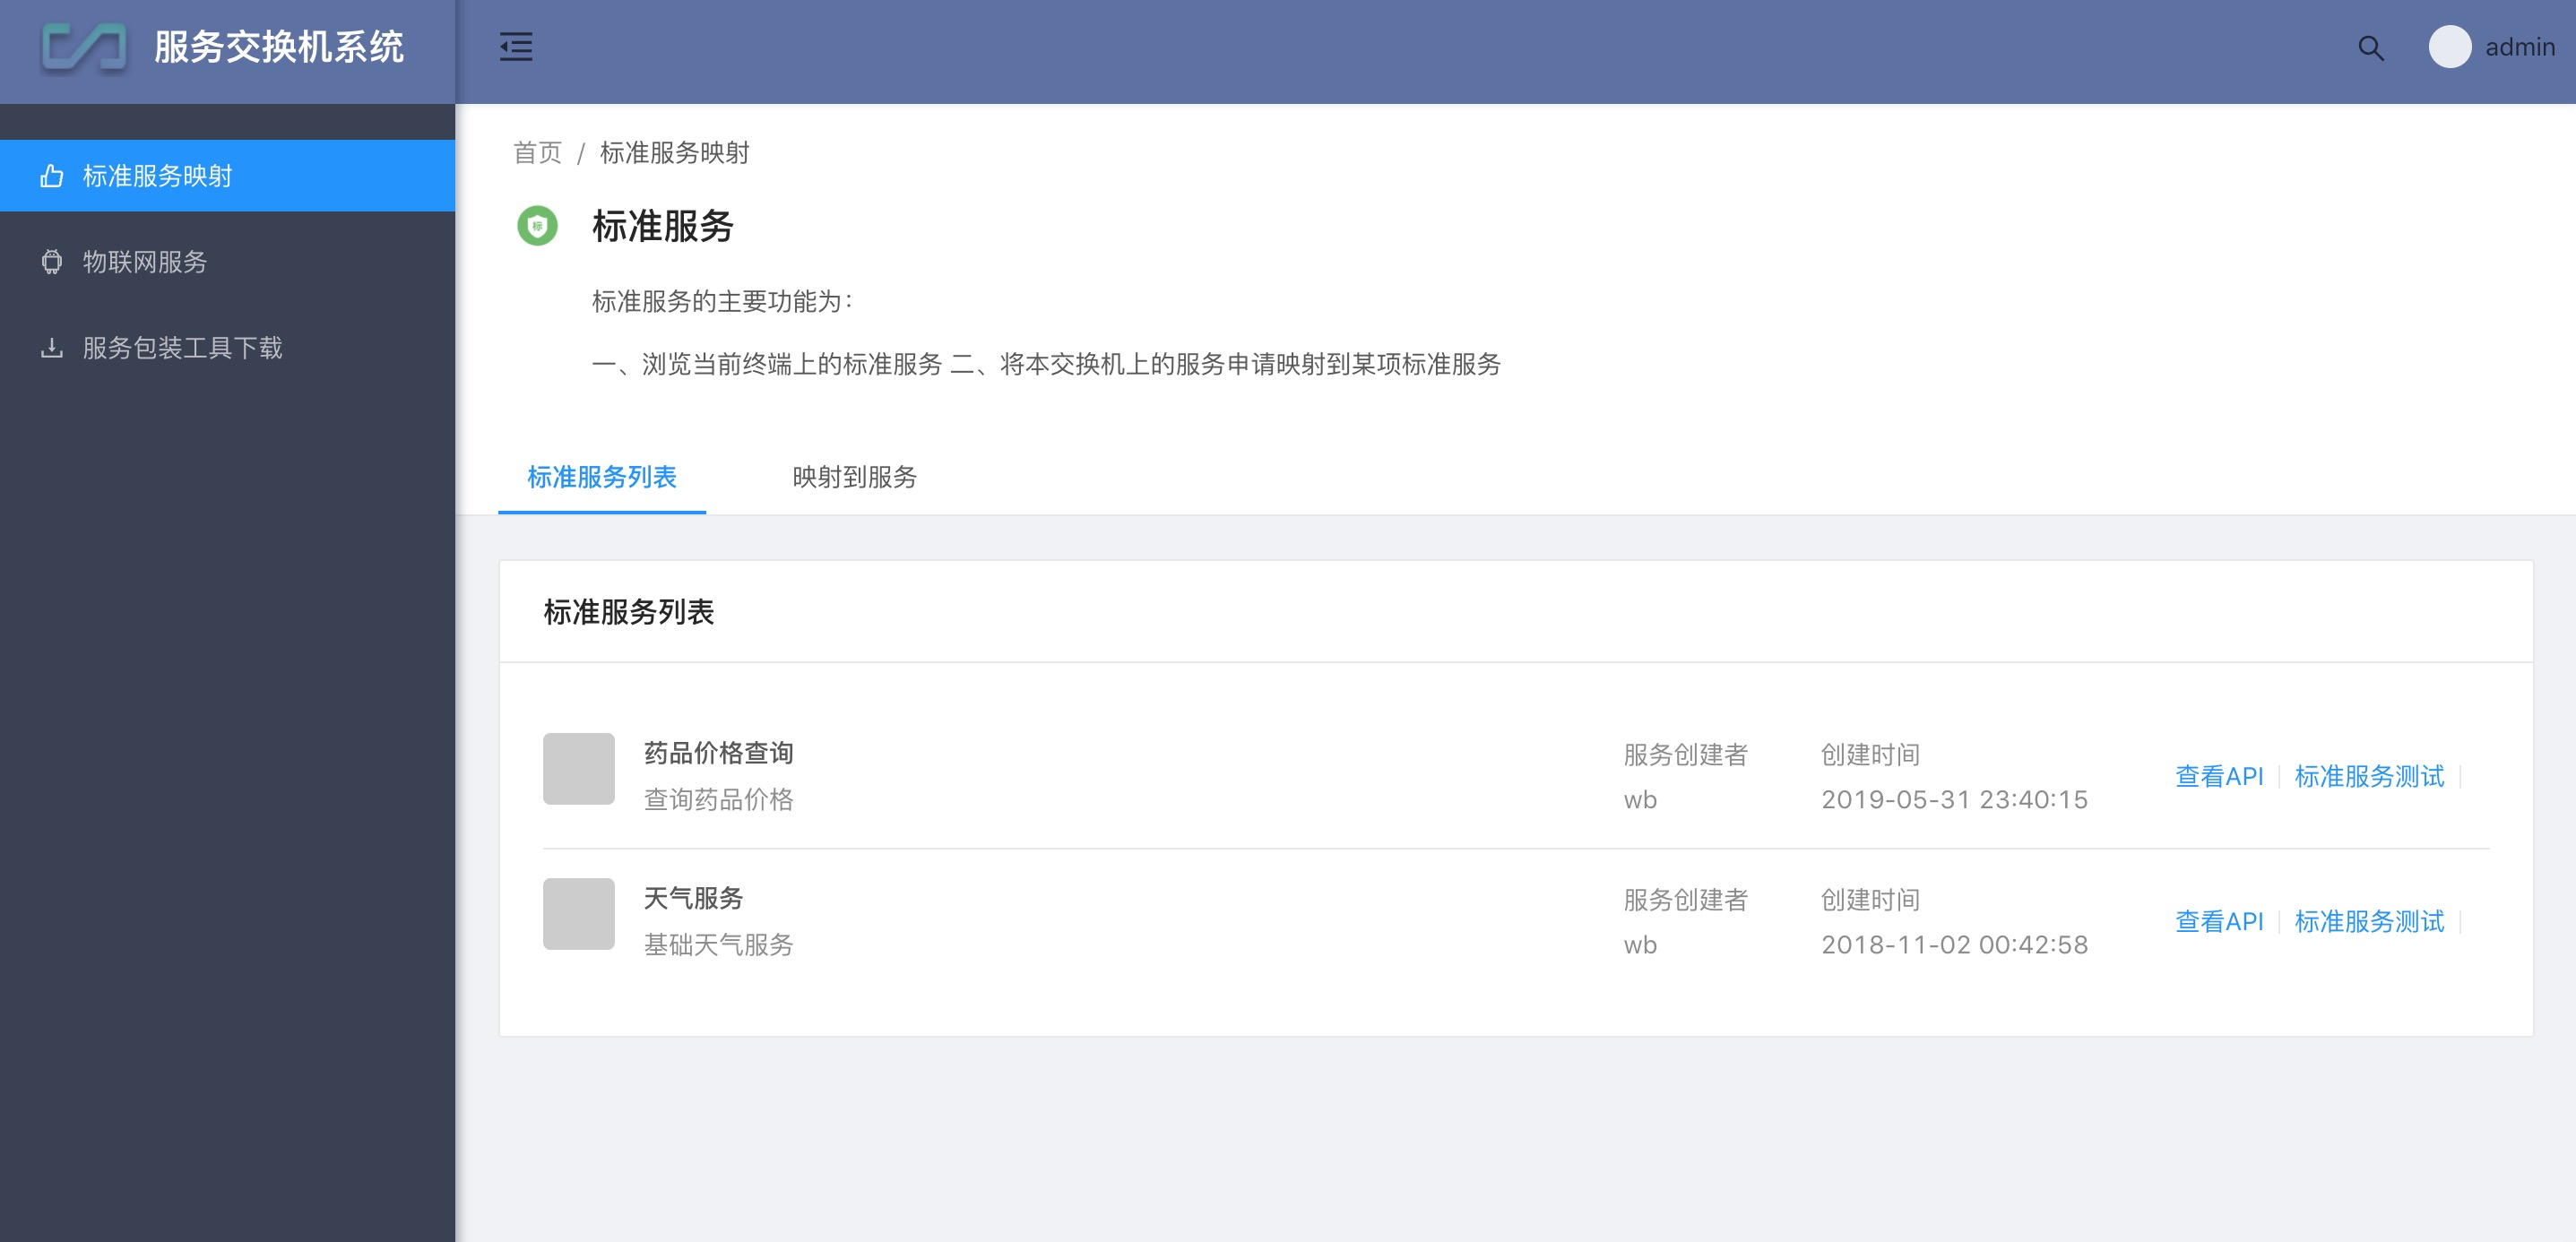
\includegraphics[width=8cm]{./images/fuwugongju1.png}
      \label{fig:fuwugongju1}
    }
    \subfloat[物联网服务]{
      \centering
    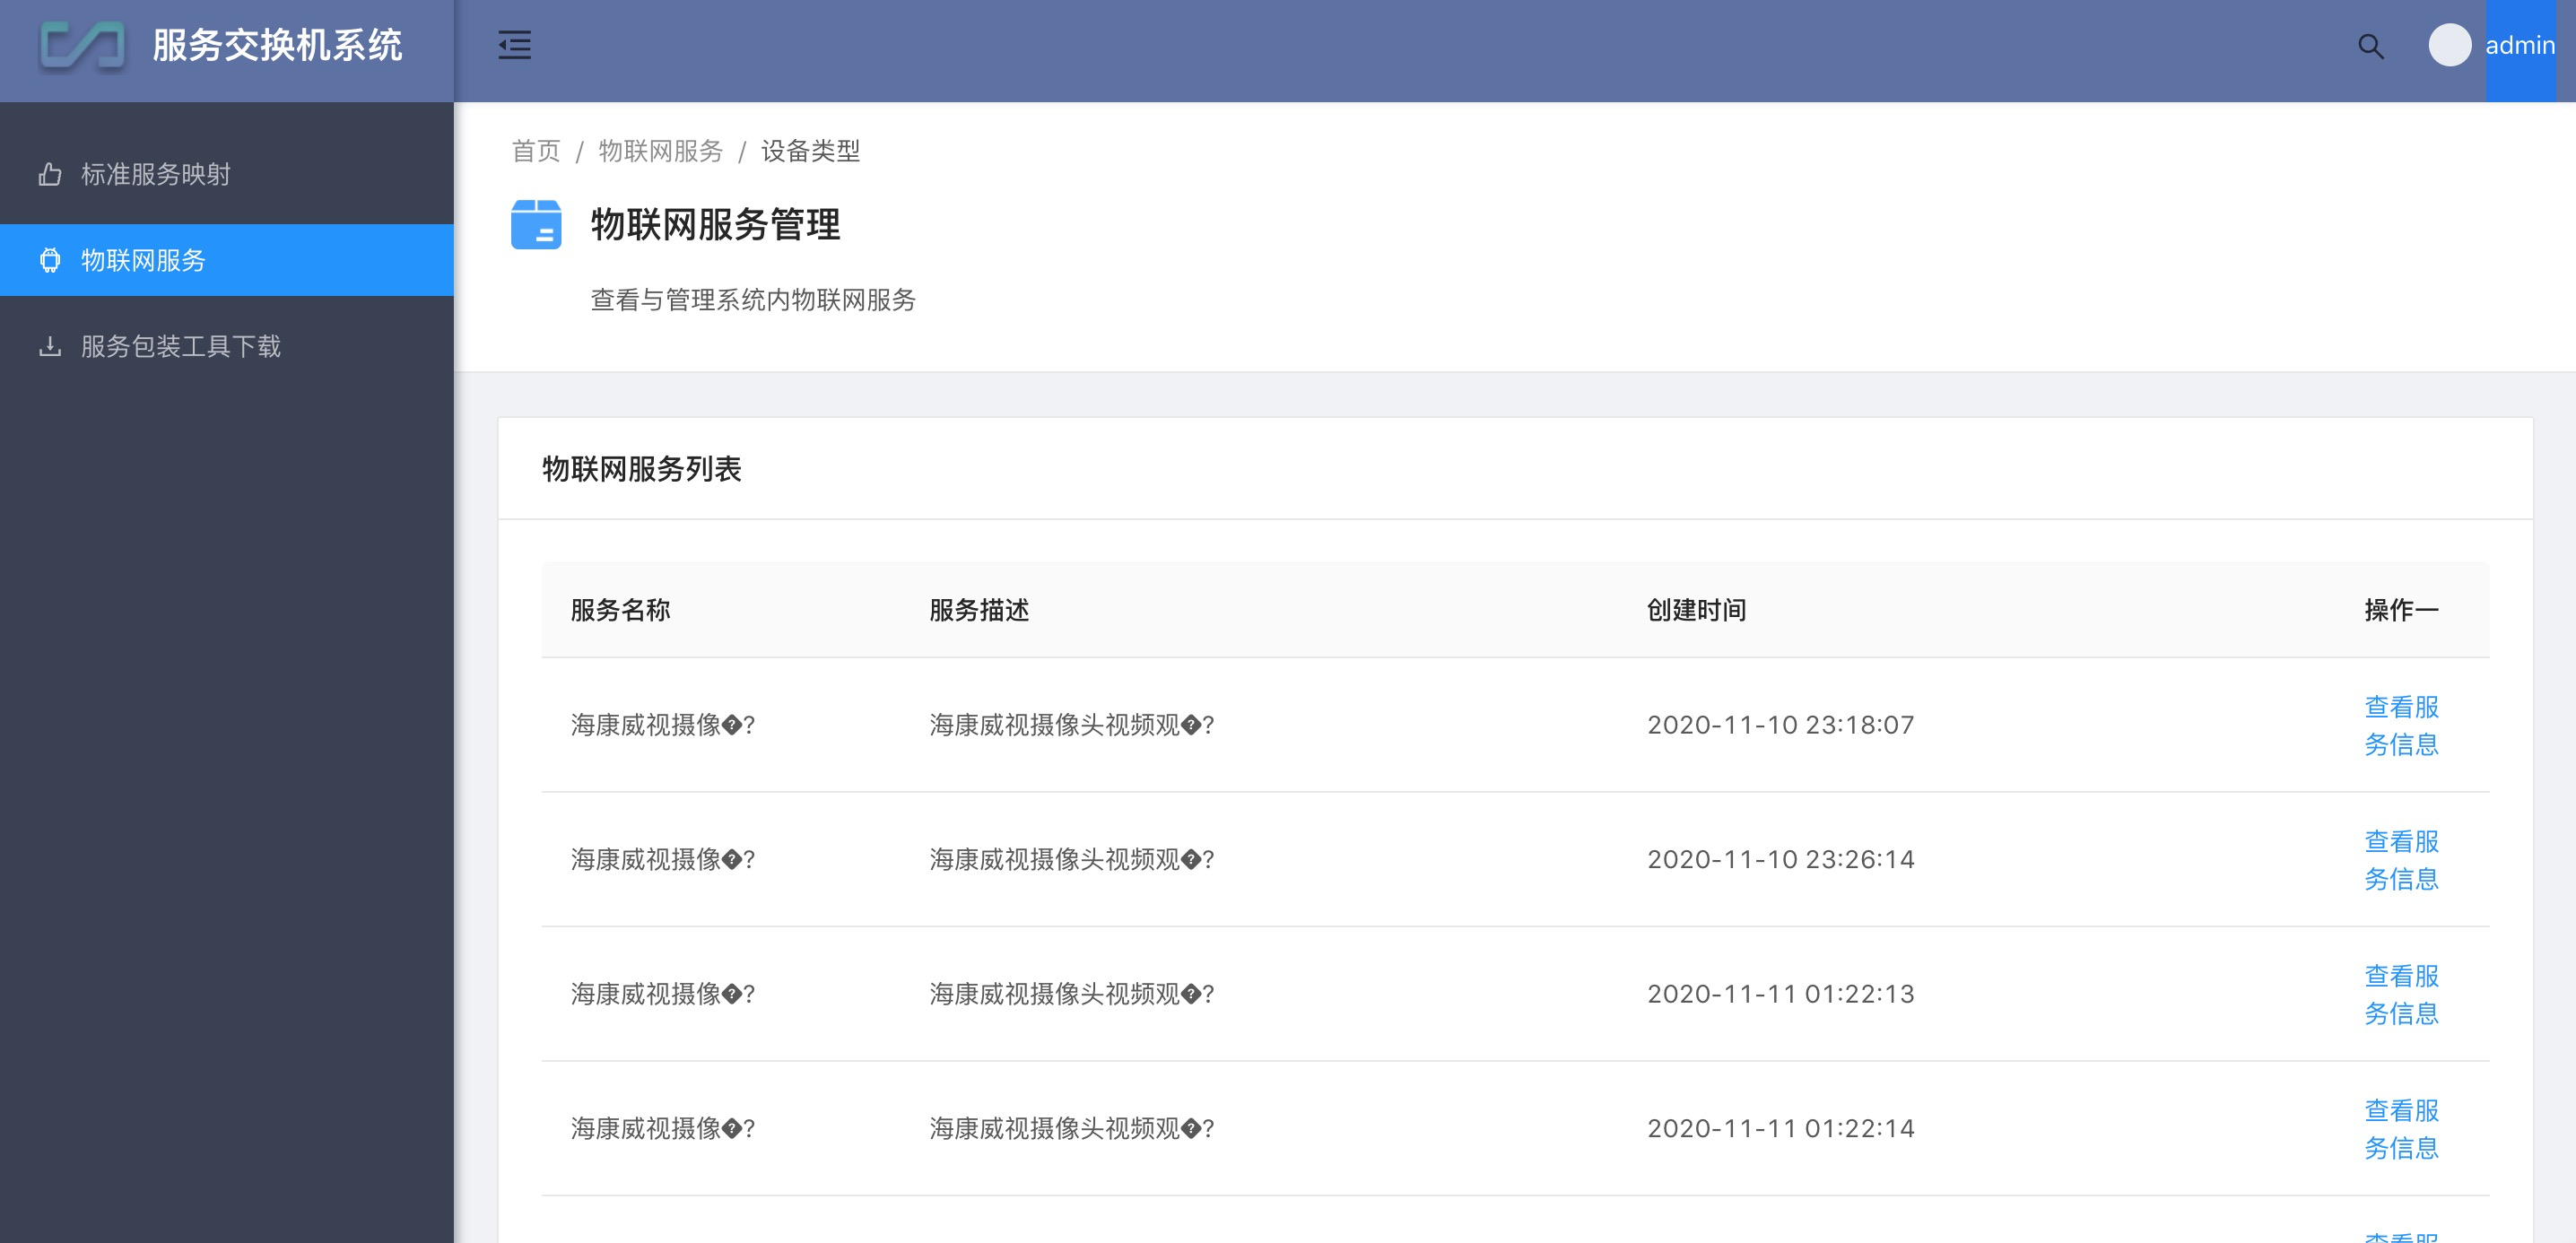
\includegraphics[width=8cm]{./images/fuwugongju2.png}
    \label{fig:fuwugongju2}
    }
    \caption{服务交换机工具模块}
    \label{fig:fuwugongju}
    \end{figure}
% \section{本章小结}